\documentclass[border=10pt]{standalone}
\usepackage{xcolor}
\usepackage{tikz}
\usetikzlibrary{positioning}

\definecolor{INK}{HTML}{1A1A2E}
\definecolor{BG}{HTML}{FAFAFA}
\definecolor{SUB}{HTML}{555566}
\definecolor{COLD}{HTML}{4361EE}
\definecolor{WARM}{HTML}{2EC4B6}
\definecolor{JOB}{HTML}{D81159}

\begin{document}
\pagecolor{BG}
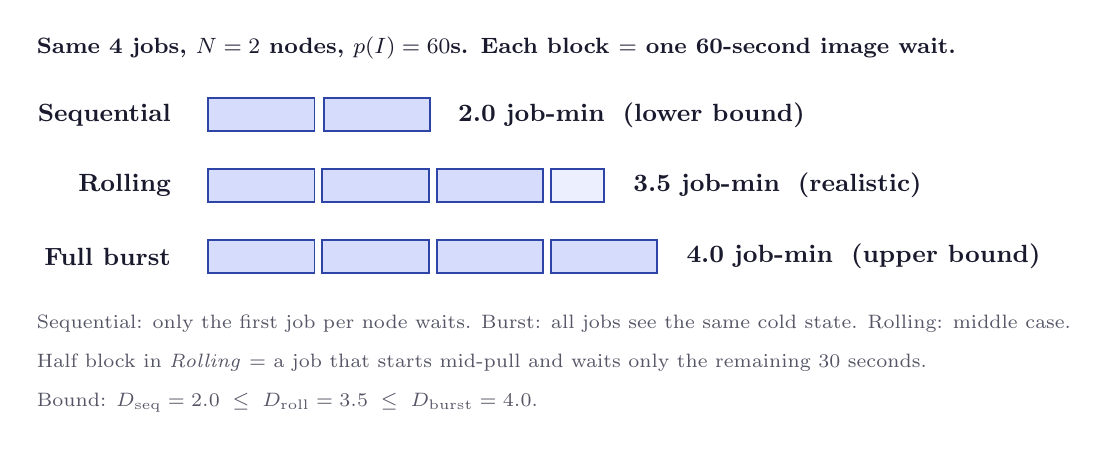
\begin{tikzpicture}[
    font=\sffamily,
    full/.style={fill=COLD!22, draw=COLD!70!black, line width=0.7pt},
    partial/.style={fill=COLD!10, draw=COLD!70!black, line width=0.7pt},
    rowlabel/.style={font=\small\bfseries, text=INK, anchor=east},
    val/.style={font=\small\bfseries, anchor=west, text=INK},
    sub/.style={font=\scriptsize, text=SUB},
    head/.style={font=\footnotesize\bfseries, text=INK},
  ]

  \def\bw{1.35}   % block width per p(I)=60s
  \def\bh{0.42}

  \node[head, anchor=west] at (-2.3, 3.55)
    {Same 4 jobs, $N=2$ nodes, $p(I)=60$s. Each block $=$ one 60-second image wait.};

  % --- Sequential ---
  \node[rowlabel] at (-0.35, 2.7) {Sequential};
  \draw[full] (0,2.7-\bh/2) rectangle (\bw, 2.7+\bh/2);
  \draw[full] (\bw+0.12, 2.7-\bh/2) rectangle (2*\bw+0.12, 2.7+\bh/2);
  \node[val] at (2*\bw+0.35, 2.7) {2.0 job-min \;(lower bound)};

  % --- Rolling ---
  \node[rowlabel] at (-0.35, 1.8) {Rolling};
  \draw[full] (0,1.8-\bh/2) rectangle (\bw, 1.8+\bh/2);
  \draw[full] (\bw+0.10, 1.8-\bh/2) rectangle (2*\bw+0.10, 1.8+\bh/2);
  \draw[full] (2*\bw+0.20, 1.8-\bh/2) rectangle (3*\bw+0.20, 1.8+\bh/2);
  \draw[partial] (3*\bw+0.30, 1.8-\bh/2) rectangle (3.5*\bw+0.30, 1.8+\bh/2);
  \node[val] at (3.5*\bw+0.55, 1.8) {3.5 job-min \;(realistic)};

  % --- Full burst ---
  \node[rowlabel] at (-0.35, 0.9) {Full burst};
  \foreach \k in {0,1,2,3} {
    \draw[full] (\k*\bw+\k*0.10, 0.9-\bh/2) rectangle (\k*\bw+\bw+\k*0.10, 0.9+\bh/2);
  }
  \node[val] at (4*\bw+0.55, 0.9) {4.0 job-min \;(upper bound)};

  % bounds note
  \node[sub, anchor=west] at (-2.3, 0.05)
    {Sequential: only the first job per node waits. Burst: all jobs see the same cold state. Rolling: middle case.};
  \node[sub, anchor=west] at (-2.3, -0.45)
    {Half block in \emph{Rolling} $=$ a job that starts mid-pull and waits only the remaining 30 seconds.};
  \node[sub, anchor=west] at (-2.3, -0.95)
    {Bound: $D_{\mathrm{seq}}=2.0 \;\le\; D_{\mathrm{roll}}=3.5 \;\le\; D_{\mathrm{burst}}=4.0$.};

\end{tikzpicture}
\end{document}
